\documentclass[11pt]{article}
\usepackage[utf8]{inputenc}	% Para caracteres en español
\usepackage{amsmath,amsthm,amsfonts,amssymb,amscd}
\usepackage{multirow,booktabs}
\usepackage[table]{xcolor}
\usepackage{fullpage}
\usepackage{lastpage}
\usepackage{enumitem}
\usepackage{fancyhdr}
\usepackage{mathrsfs}
\usepackage{wrapfig}
\usepackage{setspace}
\usepackage{calc}
\usepackage{multicol}
\usepackage{listings}
\usepackage{cancel}
\usepackage[margin=3cm]{geometry}
\usepackage{amsmath}
\newlength{\tabcont}
\setlength{\parindent}{0.0in}
\setlength{\parskip}{0.05in}
\usepackage{empheq}
\usepackage{framed}
\usepackage{xcolor}
\colorlet{shadecolor}{orange!15}
\parindent 0in
\parskip 12pt
\geometry{margin=1in, headsep=0.25in}
\theoremstyle{definition}
\newtheorem{defn}{Definition}
\newtheorem{reg}{Rule}
\newtheorem{exer}{Exercise}
\newtheorem{note}{Note}
\begin{document}
\setcounter{section}{0}
\title{Review Notes}

\thispagestyle{empty}

\begin{center}
{\LARGE \bf Summer Intern Lectures}\\
{\large Time Series Analysis Team}\\
June 2017
\end{center}
\section{Kalman filter}
\subsection{Overview?}
The Kalman filter is a technique that allows to recursively update one's beliefs of an unobserved (at least contamporaneously) variable. It usues Bayesian updating and historical data to predict a particular variable and potentially to forecast the state of said variable in the future. \newline

\begin{shaded}
  \textbf{Rocket example}\newline
  The typical example used to give intuition of the Kalman filter is that of identifying a rocket. You do not know where the rocker at times $t$ (we indicate this by $x_{t}$) is now but you have an idea, summarized in what is called a \textit{prior distribution} $p(x)$. Now, suppose you get new information about the position of the rocket, for example you get a satellite recording of it and you know it is at $y_{t}$ (the measurement itself will have some uncertainty). You ask yourself: where is the rocket at $t+1$? Having more information to answer this question, you will use both your prior and the actual location of the rocket to determine $y_{t+1}$. Putting prior and data together will give you the \textit{posterior distribution}. The posterior distribution becomes your prior on the position of the rocket of $t+1$ and so on we can continue until the rocket hits something.

 Here I steal from QuantEcon which displays this very well...
\begin{center}
 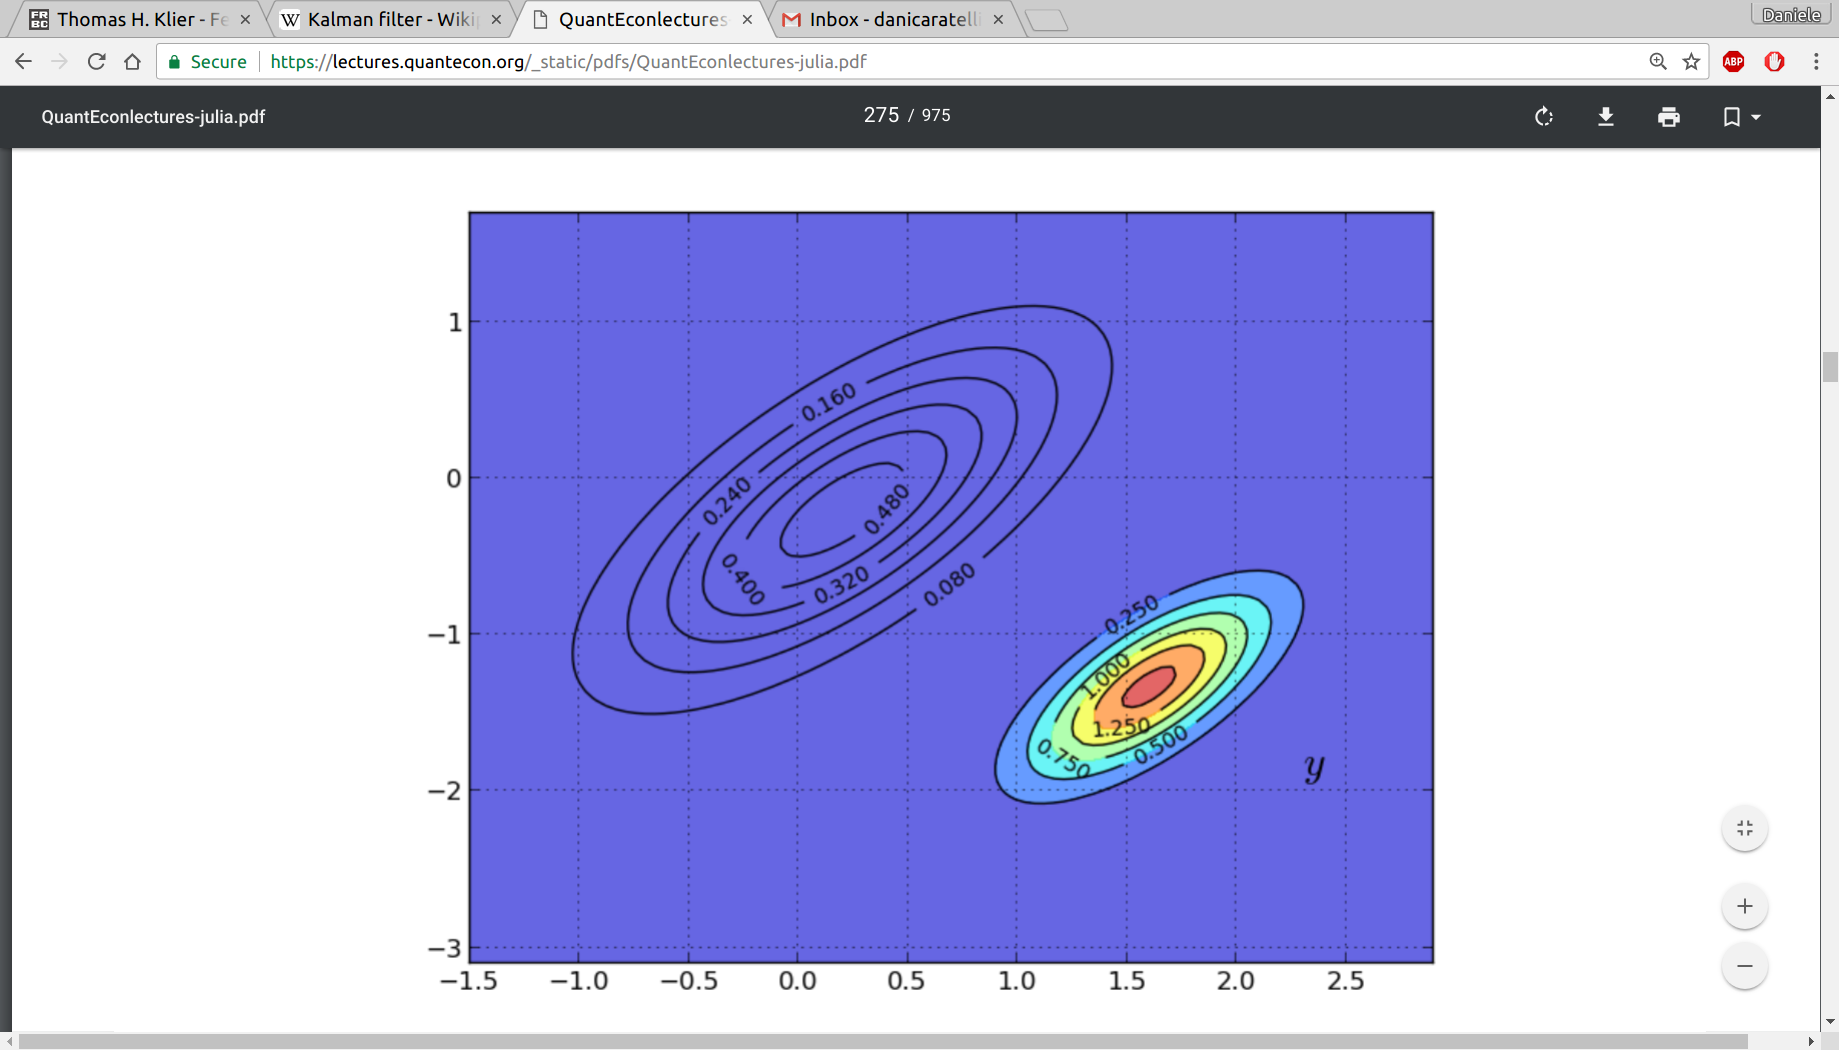
\includegraphics[scale=0.25,trim={12cm, 2cm, 12cm, 6.8cm}, clip]{plots/kalman.png}
\end{center} 
  


Notice, this relates very closely to the nowcast! As actual data comes out, we compare our \textit{prior}, i.e. the forecast, to the release and then we update our model!
\end{shaded}


\subsection{Methodology}
Here we outline the steps to run the Kalman filter.

\begin{itemize}
\item[step 1] \textbf{Prior}\newline
  Before we start we will need to have a guess (or prior) on the rocket $x$. This will be summarized in a probability distribution $p(x)$.
  \item[step 2] \textbf{Filtering}\newline
    The second step is to update our prediction after having seen the data. We receive data about the state of the rocket that can be summarized as $p(y)$ (we shall call this the likelihood, responding tot he question ``How \textit{likely} are we to see the data?''). Both our initial prior and the data are uncertain so we take both of them into account to update our beliefs. The updating process is done very simply following Bayes' law:

    \begin{equation}
      p(x|y) = \frac{p(y|x)\cdot p(x)}{p(y)}
    \end{equation}

    Where we call $p(x|y)$ the \textit{posterior} distribution which should be thought of as a weighted average between what the data suggests and your prior belifs. In particular, if the data is very noisy and your prior is very tight (i.e. you are fairly certain about the position of the rocket), the posterior will weigh your prior beliefs heavily and the data little, similarly, if the data is not noisy and your believs are flat (you are very uncertain about the position of the rocket a priori), the posterior will weigh the data more and the prior less.

    This step is called the \textit{filtering} step because it filters out the noise from the data and our prior when coming up with the posterior distribution.

\item[step 3] \textbf{Forecasting}\newline
  
  If we want to forecast the position of the rocket in the next period or the one after that we need a forecasting model that relates the position of the rocket this period with the position of the rocket next period.

An example of such model would be the following:  
  \begin{equation}
    x_{t+1} = f(x_{t}) + w_{t+1},
  \end{equation}

  this law of motion (or transition equation) should look very familiar to those who have studied state-space models, in fact, in order to run the Kalman filter, you need to put your model in state-space format!

  To get a prediction (often summarized as a whole predictive distribution) we simply put together our filtering distribution $p(y|x)$ (the posterior distribution from the filtering step) and our law of motion $f(x_{t})$. The predictive distribution will be nothing other than:

  \begin{equation}
    p(x_{t+1}) = f(p(y|x)),
  \end{equation}
(note this is not the cleanest way of writing this, but it conveys the idea).

\end{itemize}

\subsection{Summary and recursion}
Often we get multiple updates regarding the position of the rocket, at each one of these we are able to apply the two steps outlined above recursively:

\begin{lstlisting}  
  for t=1:T;
\end{lstlisting}
  \begin{itemize}
  \item Have a prior for the current period $t$, $p_{t}(x)$;
  \item Observe measurement $y_{t}$;
  \item Compute filtering distribution (posterior distribution) $p_{t}(x|y)$;
  \item Make prediction of $x_{t+1}$, $p_{t+1}(x)$ using the filtering distribution and the transition equation (this will be the prior for your next iteration).
  \end{itemize}
\begin{lstlisting}  
  end
\end{lstlisting}


\end{document}
